% !TEX root =  ../main_manuscript.tex 
\section{Introduction}

Patients with low- and very low-risk screening-detected localized prostate cancer (PCa) are usually advised active surveillance (AS) instead of immediate radical treatment \citep{briganti2018active}. In AS, PCa progression is routinely monitored via prostate-specific antigen (PSA), digital rectal examination, and the Gleason score from repeat prostate biopsies. Among these, the Gleason score is the strongest indicator of cancer related outcomes. Thus, patients are commonly advised curative treatment upon disease reclassification \citep{bul2013active}, which is detected via upgrade in biopsy Gleason score.

Since biopsies are scheduled intermittently, disease reclassification is always detected with a delay. The smaller the delay is, the larger is the window of opportunity for curative treatment. To this end, majority of the AS programs worldwide, schedule biopsies every 12-24 months for all patients \citep{nieboer2018active,loeb2014heterogeneity}. Such fixed and frequent biopsies may benefit a small proportion of men with a high risk of reclassification. However, for the majority of the \textit{slow progressing} patients frequent biopsies are redundant (see Figure \ref{fig:npmle_plot}). Biopsies are also invasive, painful and prone to medical complications. The unnecessary burden of biopsies, and the consequent patient non-compliance \citep{bokhorst2015compliance}, has raised questions about the optimal time interval between subsequent biopsies \citep{inoue2018comparative, bratt2013study}.

\begin{figure}[!htb]
\centerline{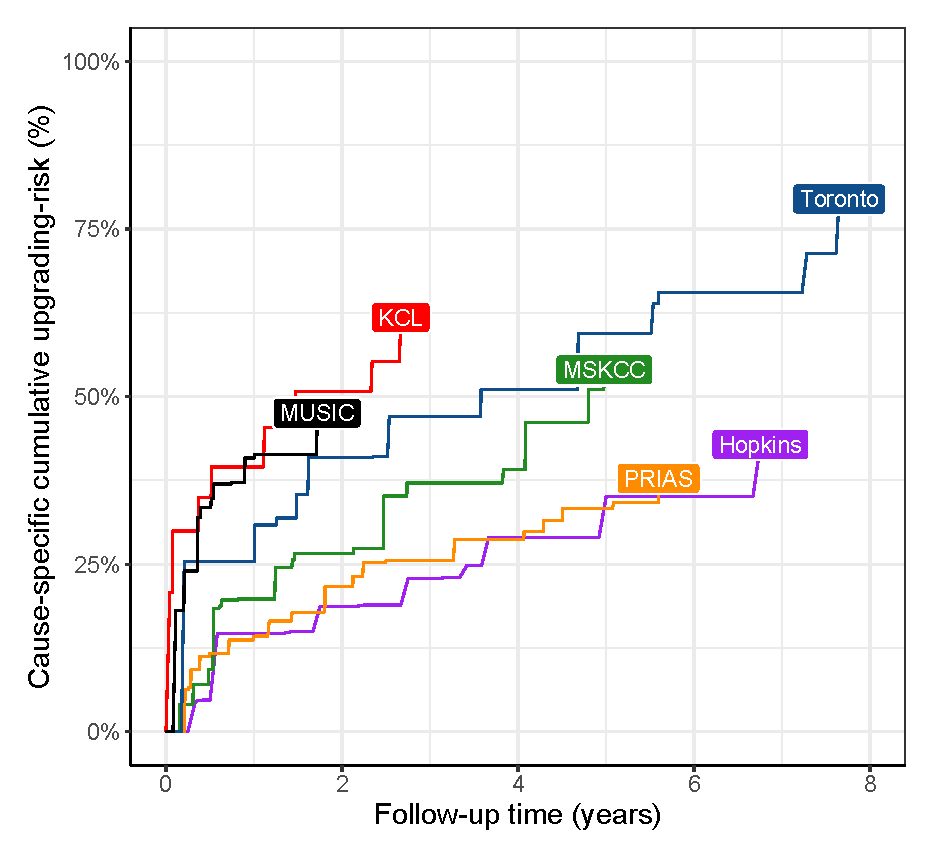
\includegraphics[width=\columnwidth]{images/npmle_plot.eps}}
\caption{\textbf{Estimated cumulative risk of reclassification in AS} for patients in the world's largest AS patient program called PRIAS. Nearly 50\% patients do not obtain reclassification in the ten year follow-up period and hence do not require a repeat biopsy. Censoring includes death, removal from AS on protocol basis, and patient dropout.}
\label{fig:npmle_plot}
\end{figure}

The simplest solution to frequent biopsies is reducing the frequency of biopsies for all patients. However, simulation studies have suggested that reducing the frequency beyond 24 months may not leave sufficient window of opportunity for curative treatment \citep{inoue2018comparative}. Although, with a gap of 24 months up to five unnecessary biopsies over ten years of follow-up may still be scheduled for the \textit{slow progressing} patients. A promising alternative to such fixed rules is biopsy decisions based on the risk of reclassification. Consider for instance the two patients shown in Figure ... Both patients had their latest biopsy at year one of follow-up and are now scheduled for a biopsy after a 24 month gap at year three. The PSA profile of patient A is stable and the PSA profile of patient B is fast rising. Since the risk of reclassification for patient A (vice-versa for patient B) is very low, he may not be subjected to unnecessary biopsy at year three.

The first challenge in the risk based approach is consolidation of observed patient data. The observed PSA levels of each patient are longitudinal in nature, may vary non-linearly over time (Figure ...), and are subject to arbitrary fluctuations \citep{ito2003natural}. In this regard, joint models for time-to-event and longitudinal data \citep{rizopoulos2012joint} have been employed to extract information from the whole PSA profile, and then to combine it with results of previous biopsies \citep{tomer2019,coley2017prediction}. This results into a patient and visit-specific dynamic risk of reclassification. A subsequent challenge however, is to translate these risk estimates into decisions, and to provide an estimate of the consequences of each decision in a personalized manner. To tackle this challenge, a complete framework for shared decision making of biopsies is required.

The goal of this work is to help patients and doctors make better decisions of biopsies than fixed and frequent biopsies. To this end, we first fit a prediction (joint) model to the world's largest AS dataset, PRIAS. Subsequently, we validate our model in multiple external cohorts that are part of the GAP3 database. Using the personalized risk predictions, we then propose the aforementioned framework for shared decision making of biopsies. Lastly, we implement the decision making framework as a web-application, and demonstrate it with real patient data.